\documentclass[xcolor=dvipsnames, utf8]{beamer}

\mode<presentation>
{
\usetheme{Ilmenau}
%\usecolortheme{Seahorse}
\setbeamercovered{transparent}
}

\usepackage[ngerman]{babel}
\usepackage[utf8]{inputenc}

\usepackage{mathptmx}
\usepackage[scaled=.90]{helvet}
\usepackage{courier}
\usepackage{hyperref}
\usepackage{BeamerColor}

\usepackage[T1]{fontenc}

\title{Entwicklung eines Web Based Training Systems nach dem Dreyfus fünf
Etappen Modell mentaler Aktivitäten}
\beamertemplatenavigationsymbolsempty

\author{Michael Gruben}

\institute[DHBW Karlsruhe und Meyle+Müller GmbH+Co. KG]{Duale Hochschule
Baden-Württemberg Karlsruhe \and Meyle+Müller GmbH+Co. KG}

\date{17. September 2013}

\subject{\title}

\usepackage{colourchange}
\graphicspath{{images/}}

\pgfdeclareimage[height=0.5cm]{mum-logo}{images/mum.png}
\logo{\pgfuseimage{mum-logo}}

\AtBeginSection[]
{
\begin{frame}<beamer>
\frametitle{Gliederung}
\tableofcontents[currentsection,hidesubsections]
\end{frame}
}

\AtBeginSubsection[]
{
\begin{frame}<beamer>
\frametitle{Gliederung}
\tableofcontents[currentsection,subsectionstyle=show/shaded/hide]
\end{frame}
}

\begin{document}
\selectmanualcolour{DodgerBlue3}
\beamerdefaultoverlayspecification{<+->}
\begin{frame}
\titlepage
\end{frame}

\begin{frame}
\frametitle{Gliederung}
\tableofcontents[hideallsubsections]
\end{frame}

\section{Über das Projekt}
\begin{frame}
\frametitle{Eckdaten}
 \begin{itemize}
   \item Studienarbeit an der DHBW Karlsruhe
   \item Zusammenarbeit von\begin{itemize}
     \item Julian Babics (MedicalCommunications Soft- und Hardware GmbH,
     Bruchsal)
     \item Benjamin Merkle (SAP AG, Walldorf)
     \item Michael Gruben (Meyle+Müller GmbH+Co.KG, Pforzheim)
   \end{itemize}
	\item Bearbeitungszeitraum: 3 Monate
 \end{itemize}
\end{frame}

\begin{frame}
\frametitle{Kontext im Studienverlauf}
\begin{itemize}
  \item Vorangegangene Studienarbeit: "`Analyse und Vergleich von
  Autorensystemen für ein WBT zu Vorlesungsinhalten"'
  \item Konzept entwickelt in der Vorlesung "`Gamification"'
\end{itemize}
\begin{block}{Zusammensetzung}
Vermischung von eLearning und Gamification
\end{block}
\end{frame}

\section{Theorie}
\subsection{Idee}
\begin{frame}
\frametitle{Prinzip}
\begin{itemize}
  \item offene und gesellschaftliche Lernplattform
  \item Lernende treffen auf Lehrende
  \item Anwenden des Dreyfus fünf Etappen Modells mentaler Aktivitäten
  \item nur Meister sind Autoren neuer WBTs
  \item Realisieren von Blended Learning
  \item Aufnehmen gamifizierender Elemente
  \item Namensgebung: "`Masterly Mate"'
\end{itemize}
\end{frame}
\begin{frame}
\frametitle{Stichworte}
\centering
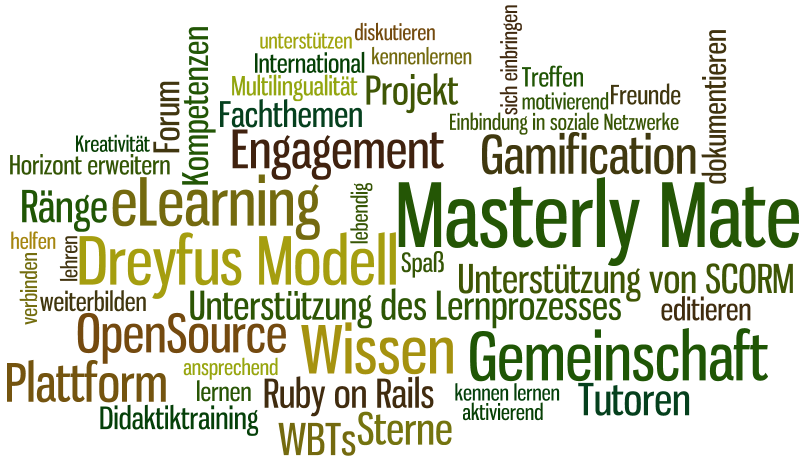
\includegraphics[width=0.9\textwidth]{MasterlyMateWolke.png}
\end{frame}
\subsection{Komponenten}
\begin{frame}
\frametitle{Learning Management System}
\begin{itemize}
  \item wird als Lernplattform bezeichnet
  \item bekannter Vertreter ist Moodle
  \item organisiert Lernstoff in Kursen
  \item oft können Web Based Trainings eingebettet werden
\end{itemize}
\end{frame}
\begin{frame}
\frametitle{Dreyfus fünf Etappen Modell mentaler Aktivitäten}
\begin{block}{Zweck}
Zuordnung eines geeigenten Lehrers zu einem Lernenden auf entsprechendem Niveau
\end{block}
\begin{itemize}
  \item fünf Etappen\begin{itemize}
    \item Novize
    \item Fortgeschrittener
    \item Erfahrener
    \item Experte
    \item Meister
  \end{itemize}
\end{itemize}
\end{frame}
\begin{frame}
\frametitle{Blended Learning}
\begin{itemize}
  \item zu Deutsch "`Integriertes Lernen"'
  \item Verschmelzen von Präsenzveranstaltungen, entferntem Lernen und eLearning
\end{itemize}
\begin{block}{Zweck}
Es vereint die jeweiligen Vorteile und überwindet die Nachteile der Methoden 
\end{block}
\end{frame}

\subsection{Anwendungsfall}
\begin{frame}
\frametitle{Lernender eignet sich Fachkenntnis an oder erweitert sie}
\begin{columns}
\begin{column}{7cm}
\begin{enumerate}
  \item Login
  \item Wahl eines Kurses auf seinem Niveau\begin{enumerate}
    \item Wahl des Fachbereichs
    \item Wahl des WBTs
    \item Öffnen des Kurses im SCORM-Player
  \end{enumerate}
  \item Bearbeiten des Kurses\begin{description}
    \item[Fall A] es wird keine Hilfe benötigt
    \item[Fall B] es wird Hilfe benötigt
  \end{description}
\end{enumerate}
\end{column}
\begin{column}{3cm}
\only<3>{
\includegraphics[width=3cm]{Key.png}}
\only<4-7>{
\includegraphics[width=3cm]{studentbooks.png}}
\only<8-11>{
\includegraphics[width=3cm]{lampe.png}}
\end{column}
\end{columns}
\end{frame}

\begin{frame}
\frametitle{Fall A -- es wird keine Hilfe benötigt}
\begin{columns}
\begin{column}{7cm}
\begin{enumerate}
  \setcounter{enumi}{3}
  \item Absolvieren des WBTs und Wertung\begin{description}
  \item[bei Bestehen] werden fachliche Punkte des eigenen Rangs erhöht
  \item[bei nicht Bestehen] werden bleiben sie gleich\end{description}
  \item[optional] Bewerten des WBTs
  \item Bearbeiten weiterer WBTs oder Logout
\end{enumerate}
\end{column}
\begin{column}{3cm}
\only<3-5>{
\includegraphics[width=3cm]{award.png}}
\only<6>{
\includegraphics[width=3cm]{thumbUp.png}}
\only<7-8>{
\includegraphics[width=3cm]{logout.png}}
\end{column}
\end{columns}
\end{frame}

\begin{frame}
\frametitle{Fall B -- es wird Hilfe benötigt}
\begin{columns}
\begin{column}{7cm}
\begin{enumerate}
  \setcounter{enumi}{3}
  \item die Hilfe eines Tutors wird angefordert\begin{enumerate}
    \item Klick auf Hilfe anfordern
    \item geeigneten Tutor aus gefilterter Liste wählen
    \item Tutor kontaktieren
    \item[optional] mit Tutor treffen
    \item Tutor bewerten
  \end{enumerate}
  \item weiter, wie in Fall A
\end{enumerate}
\end{column}
\begin{column}{3cm}
\only<3-8>{
\includegraphics[width=3cm]{Help.png}}
\only<9-10>{
\includegraphics[width=3cm]{reload.png}}
\end{column}
\end{columns}
\end{frame}

\section{Praxis}
\subsection{Entwurf}
\begin{frame}
\frametitle{Technische Sicht}
\begin{itemize}
  \item Webapplikation
  \item Ruby on Rails
  \item Prototyp
  \end{itemize}
  \begin{block}{Zielsetzung}
  Jeder soll auf die Applikation zugreifen oder sich bei Interesse an der
  Weiterentwicklung beteiligen können!
  \end{block}
  \end{frame}
  
\begin{frame}
  \frametitle{Organisatorische Sicht}
  \begin{itemize}
  \item Wertlegung auf\begin{itemize}
    \item Erweiterbarkeit
    \item Offenheit
    \item Internationalisierung
  \end{itemize}
  \item Gewählte Lizenz: AGPL\footnote{Affero GNU General Public License}
  \item Modellieren von Anwendungsfällen
\end{itemize}
\end{frame}

\subsection{Umsetzung}
\begin{frame}
\frametitle{Frontend}
\begin{itemize}
  \item Nutzerverwaltung inklusive Authentifizierung
  \item Übersicht über vorhandene WBTs\footnote{Web Based Trainings},
  organisiert in Themen
  \item Betrachtung von WBTs im SCORM\footnote{Shared Content Object
  Reference Model}-Format
  \item Beachtung von Usability-Aspekten
  \end{itemize}
  \end{frame}
  
\begin{frame}
\frametitle{Screenshot}
\centering
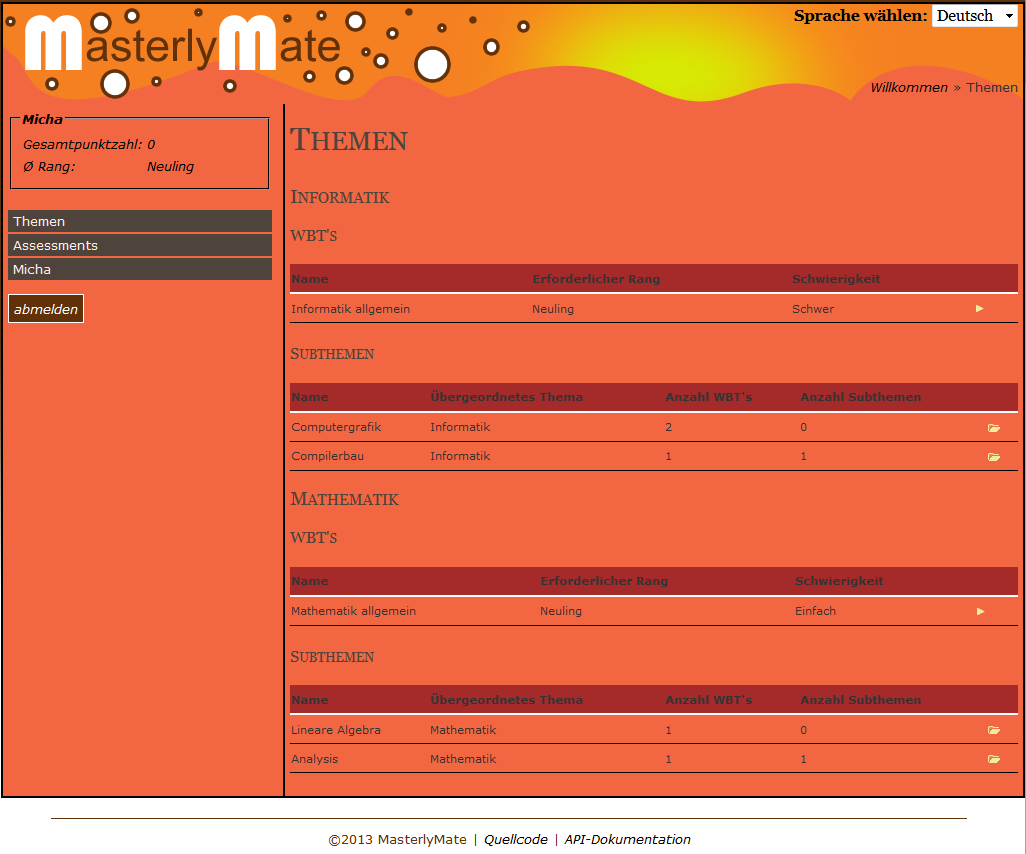
\includegraphics[width=0.6\textwidth]{ScreenshotThemen.PNG}
\end{frame}
  
\begin{frame}
  \frametitle{Backend}
  \begin{itemize}
  \item Zählen von Punkten und Übergänge zwischen Rängen vorbereitet
  \item Mechanismen zur Umsetzung einer Internationalisierung
  \item Möglichkeit zum Verwalten von WBTs im SCORM-Format  
\end{itemize}
\end{frame}

\section{Auswertung}
\subsection{Ausblick}
\begin{frame}
\frametitle{Vom aktuellen Stand zur nächsten Version}
\begin{itemize}
  \item Anwendung ist noch in Entwicklung, bisher keine produktive Version
  \item Helfende Hände werden gesucht
  \item jeder hat die Möglichkeit, sich am Projekt per Github zu beteiligen
  \item Endgültige Programmiersprache noch offen
\end{itemize}
\end{frame}

\begin{frame}
\frametitle{Noch zu entwickelnde Komponenten}
\begin{itemize}
  \item Übersicht über bereits absolvierte WBTs
  \item Upload eines Profilbildes
  \item Implementierung jährlicher Tests
  \item Rangverlust für Tutoren
  \item Quickstart
  \item Login mithilfe von Open-ID
  \item Newsletter
  \item Realitätsnahe Tests
  \item \ldots
\end{itemize}
\end{frame}

\subsection{Zusammenfassung}

\begin{frame}
\frametitle{Fazit}
\begin{itemize}
  \item Konzept vollständig, jedoch nicht final
  \item Prototyp bildet nur den Kern der Idee ab
  \item weitere Überarbeitungen und Erweiterungen notwendig
\end{itemize}
\end{frame}

\begin{frame}
\frametitle{Links}
\begin{itemize}
  \item Quellcode: \url{https://github.com/dasBKB/WBTS}
  \item Applikation auf Heroku: \url{http://pacific-gorge-6894.herokuapp.com/}
\end{itemize}
\end{frame}

\section*{}
\begin{frame}
\centering

\includegraphics[width=0.9\textwidth]{mm_header.png}\\
\Huge{Vielen Dank für die Aufmerksamkeit}\\
\Large{Anteilnahme ist erwünscht}
\end{frame}

\end{document}